\begin{figure}[ht]
   \centering
   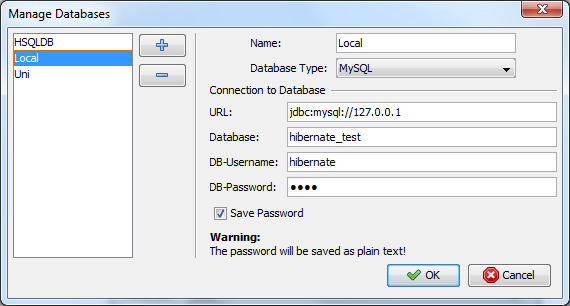
\includegraphics[scale=0.8]{images/sh_databases_dialog.png}
   \caption{Databases Dialog}
   \label{fig:databases_dialog}
\end{figure}

You can select the database to work with using the drop-down box in the \guidialog{Start Dialog}.
To add a new database to this list, click on the \gui{Databases} button.
This opens the \guidialog{Databases Dialog} shown in \figref{fig:databases_dialog}.
On the left hand side of the window, the existing database connections are shown.
With the plus and minus buttons you can create a new connection or remove an existing one.
On the right hand side the settings for the selected database are shown.

The name is only used for identification of the database connection -- you can enter any name in this field.

\gui{Database Type} is used to define the database system. At the moment \sh supports two different types of databases: \hsqldb and \mysql.

A \hsqldb database is an internal and local database.
As it is easy to configure, this database is best if you want to test \sh or to have a small private database.
If you choose a \hsqldb database, the only setting left is the database path, where you can specify a location to store the database.

\mysql is a server-based database.
It requires a \mysql server that may be running on the same machine as \sh, or on a different machine.
To configure a \mysql connection, there are a few settings to be made.
The \gui{URL} field holds the server name or IP address.
For example, ``localhost'' or ``127.0.0.1'' both would point to the local machine.
The protocol name ``jdbc:mysql://'' is not necessary and will be added automatically.
In the \gui{Database} field the database or schema name is entered.
Please note that if an existing database is entered not containing tables created
by \sh, you will be asked if you want to overwrite all existing data when connecting
to the database for the first time.
The \gui{DB Username} is used to log in to the database.
This user must be configured on the \mysql server and needs all rights to manipulate data in the database, see~\secref{sec:scaffoldhunter:requirements:database} for further information on database and user account creation.
The connection to the database also requires a password, which can be saved in the configuration file.
Please note that password is stored unencrypted.
If this password is not saved, you will be asked to enter the password each time you log in to the database.
